27. а) $f(x)=\cfrac{x-2+|2x-1|}{x^2-1}=\begin{cases}\cfrac{3x-3}{(x-1)(x+1)},\ x\geqslant\cfrac{1}{2},\\ \cfrac{-x-1}{(x-1)(x+1)},\ x<\cfrac{1}{2}.\end{cases}=
\begin{cases}\cfrac{3}{x+1},\ x\geqslant\cfrac{1}{2},\ x\neq1,\\ \cfrac{1}{1-x},\ x<\cfrac{1}{2},\ x\neq-1.\end{cases}$
$$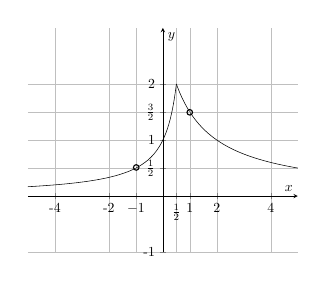
\begin{tikzpicture}[scale=0.5]
\begin{axis}[
    axis lines = middle,
    grid=major,
    legend pos={south west},
    xlabel = {$x$},
    %xlabel style={below right},
    ylabel = {$y$},
    ymin=-1,
    ymax=3,
    xtick={-4, -2,-1,0.5,1, 2,4},
    xticklabels={-4, -2,$-1$,$\frac{1}{2}$, 1, 2, 4},
    ytick={-1,0.5, 1, 1.5, 2},
     yticklabels={-1,$\frac{1}{2}$, 1, $\frac{3}{2}$, 2},
                  ]
	\addplot[domain=-5:-1.01, samples=100, color=black] {1/(1-x)};
    \addplot[domain=-0.99:0.5, samples=100, color=black] {1/(1-x)};
    \addplot[domain=0.5:0.99, samples=100, color=black] {3/(x+1)};
    \addplot[domain=1.01:5, samples=100, color=black] {3/(x+1)};
    %\addlegendentry{$\text{Рис. 1}$};
\end{axis}
\draw (2.75,2.15) circle (2pt);
\draw (4.11,3.55) circle (2pt);
\end{tikzpicture}$$
б) По графику определим $D(f)=(-\infty;-1)\cup(-1;1)\cup(1;+\infty),\ E(f)=(0;2].$\\
в) По графику определим количесво решений: $a\in(-\infty;0]\cup(2;+\infty):0,\ a\in\left\{\cfrac{1}{2}; \cfrac{3}{2},2\right\}:1,\ a\in\left(0;\cfrac{1}{2}\right)\cup\left(\cfrac{1}{2};\cfrac{3}{2}\right)\cup\left(\cfrac{3}{2};2\right):2.$\\
